% Beyond the Lean code Code Alone -- TMLR preprint style. Compile: latexmk -pdf main_en.tex
\documentclass[10pt]{article}
\usepackage[preprint]{tmlr}
\usepackage[utf8]{inputenc}
\DeclareUnicodeCharacter{2212}{\ensuremath{-}}
\usepackage{amsmath,amssymb,mathtools}
\usepackage{booktabs,tabularx,array,graphicx}
\usepackage[shortlabels]{enumitem}
\usepackage{xcolor}
\definecolor{tinta}{HTML}{4F4086}
\usepackage[colorlinks=true,linkcolor=black,citecolor=tinta,urlcolor=tinta]{hyperref}
\usepackage{url}
\usepackage{upquote}   % acentos graves rectos en el bloque verbatim del prompt
\newcommand{\vr}[1]{\texttt{#1}}
\newcommand{\D}{\Delta}
\newcommand{\ic}[2]{[#1,\,#2]}
\newenvironment{idea}{\begin{quote}\noindent}{\end{quote}}
\newenvironment{pendiente}{\begin{quote}\small\noindent\textbf{Pending.}\ }{\end{quote}}

\title{Beyond the Lean code Code Alone: Do Frozen Language Models Linearly Separate Faithful from Unfaithful Lean~4 Formalizations?}

\author{\name Carlos Manuel Orrego-Franco \email corregof@unal.edu.co \\
      \addr Departamento de Matem\'aticas y Estad\'istica\\
      Universidad Nacional de Colombia, Manizales
      \AND
      \name Juan Carlos Ria\~no-Rojas \email jcrianoro@unal.edu.co \\
      \addr Universidad Nacional de Colombia, Manizales
      \AND
      \name Fabi\'an Fernando Serrano-Su\'arez \email ffserranos@unal.edu.co \\
      \addr Universidad Nacional de Colombia, Manizales}

\begin{document}
\maketitle

\begin{abstract}
A Lean formalization can compile and still say something other than the statement it was meant to capture.
We ask whether the activations of frozen language models linearly separate faithful from unfaithful Lean~4
formalizations \emph{beyond what the Lean code alone gives away}. We measure, at three levels, the AUROC gap
between a linear probe reading the statement with the formalization and one reading the formalization alone.
No level alone supports the claim that faithfulness is linearly decodable from frozen models beyond the Lean code alone.
On 450 CriticLeanBench formalizations a preregistered replication did not pass, because none of its four models
met the per-model criterion. A post hoc bootstrap puts their mean gap at +0.045 (95\% CI \ic{0.021}{0.069}) at a
fixed layer, whereas at the last token the interval includes zero.
On 377 minimal pairs certified by Lean, exploratory runs gave a positive gap in three of four models at the last
token, but against the stronger of two surface controls only one keeps a margin whose interval excludes zero.
At that level, shifting activations along the separating axis changes the model's answer more than random
directions do in two of four models, one of them in a post hoc run.
On ProofNetVerif the gap was positive in two models, one of them exploratory.
Exploratory maps place the separation over the Lean tokens, in the upper layers.
We outline a confirmatory test on statements written
after the models' release and after this pilot.
\end{abstract}

\section{Introduction}

A proof assistant checks that a proof follows from a statement, but whether the statement is the one we meant lies
outside its reach. When a language model translates ``every bounded monotone sequence converges'' into Lean~4, the
kernel will accept any well-typed proposition, including one that drops the boundedness hypothesis or quantifies
over the wrong set. As autoformalization scales, errors of this kind can hide wherever a statement compiles and is
not the one intended.
The problem is now visible at scale. Of some 290 Lean-bearing papers in a recent batch of AI-generated mathematics, about
38 do not state the paper's main theorem \citep{xena2026checked}, and a proof checked in Lean need not match the
written argument it accompanies \citep{bastounis2026lost}.

The experiment is simple to state. We show a frozen language model a natural-language statement and a Lean~4
formalization of it, and ask: ``Is this formalization faithful? Answer Yes or No.'' We keep its answer as a control.
What we study is its activations, on which we train a linear probe to separate faithful from unfaithful
formalizations. We then repeat the run with the statement removed, so that the model sees only the Lean code and the
same question. That second question has no answer, because nothing in the prompt says what the code was meant to
capture. The probe trained there therefore measures something else, namely whatever the Lean code gives away on its
own through style, length or vocabulary. For that reason we never report the AUROC of one probe taken on its own.
Every result is a gap, the AUROC of the probe that reads the statement with the Lean code minus that of the probe that
reads the Lean code alone. A positive gap is evidence that the representation carries information about the
\emph{relation} between the two texts.

Most work measures faithfulness from the outside. It relies on a judge model
\citep{criticlean,formalalign,zhang2026beyondcompilation,wang2026formalrx}, on a round trip back to natural language
\citep{amrollahi2026roundtrip}, or on an equivalence check against a reference formalization
\citep{proofnetverif,mohammad2026faithfulnessgap}. We look inside instead. Our question is whether a frozen model,
one that was never trained to judge formalizations, already carries a linearly decodable signal that distinguishes a
faithful formalization from an unfaithful one.

We say ``separates'' and ``is linearly decodable'' throughout, because a linear probe is correlational. That a
direction separates two classes does not show that the model uses it.

\paragraph{Contributions.}
\begin{enumerate}
\item A three-level design in which each level removes a confound of the previous one. Level~A has human-validated
labels on a public benchmark. Level~B has minimal pairs with Lean-certified non-equivalence and the same statement
in both members. Level~C has an independently labelled benchmark with a transfer test.
\item A \emph{cross-surface} control, built from features that cross the statement and the formal text. In the
model where we split by kind of edit, it matches the activations on numeral changes, which a Lean-only surface
baseline would have missed. Overall, however, plain n-grams of both texts are the stronger control on our pairs.
\item A preregistered replication. No model met its per-model criterion, although the mean gap of the four models
is positive under the fixed-layer readout.
\item Dating of every Level~B origin against each model's release, and a draft confirmatory protocol restricted to
statements written afterwards (Appendix~\ref{app:protocolo}).
\item Exploratory layer-by-position maps of the probe direction in five models, an analysis in the spirit of
information-based mapping \citep{searchlight}. They show where the label is linearly readable with and without the
statement.
\item An intervention at Level~B that shifts the mean over Lean tokens along the difference of class means. It changes
the model's answer more than random directions do in Qwen3-4B, where the run is post hoc, and in OLMo-2, under a rule
fixed in advance. Under the same rule it does not meet the criterion in Llama-3.1 or in Gemma-3.
\end{enumerate}

Table~\ref{tab:conjunta} gives the status of the evidence at each level.

% ------------------------------------------------------------------ 2
\section{Related work}

\paragraph{Closest prior work.}
The work closest to ours is that of \citet{genv}, who train a generative verifier for autoformalization into
SMT-LIB, distilled from a Z3 equivalence oracle. They name the failure we study, translations that execute and
match the expected verdict but are still wrong, and they also read their verifier from the inside. A linear probe
on sparse-autoencoder codes of its residual stream reaches 0.960 AUROC, and probes on the hidden states of their
fine-tuned baselines separate better than those baselines' outputs. Their models, however, are trained to judge,
and their setting is logic problems in SMT-LIB. Ours are frozen models that were never trained for the task, and
the formal language is Lean~4. We also measure every result against what the formal text alone separates at the
level of representations.

\paragraph{Faithfulness measured from the outside.}
The work that measures faithfulness from the outside also supplies two of our benchmarks.
FormalAlign \citep{formalalign} scores the alignment between a statement and its formalization with a model trained
for that purpose. CriticLean \citep{criticlean} trains a critic to judge Lean~4 formalizations and introduces
CriticLeanBench, which we use at Level~A. \citet{proofnetverif} study evaluation metrics for statement
autoformalization and release ProofNetVerif, which we use at Level~C.

\paragraph{Hidden states and correctness.}
Decoding correctness from hidden states has precedent. Truth-like properties are linearly decodable in natural
language \citep{geometry}, although such probes need not generalise across datasets \citep{orgad}. Code correctness
has likewise been decoded from hidden states before generation \citep{dicicco}. We therefore do not claim as ours
the observation that a model's internals can separate more than its output expresses. Our Lean-only baseline plays
the role that length and surface controls play in that literature.

\paragraph{Decodable is not used.}
\citet{decodability} probe logical validity in five open-weight models and, in three of them, test
whether intervening on the decoded information changes behaviour. We read our probing results under the warning in their title. The only causal evidence in this paper is the
intervention at Level~B, which meets its criterion in two of four models, one of them post hoc.

\paragraph{A note on terms.}
``Faithfulness'' also names the fidelity of chain-of-thought explanations. Here it means only that a formalization
states what the natural-language statement states.

% ------------------------------------------------------------------ 3
\section{Method}

\paragraph{Probe.}
For each model, layer and prompt variant we read residual-stream activations from the frozen model and fit a
standardised logistic regression ($C = 1$). All scores are out-of-fold, with folds grouped so that no statement
appears on both sides of a split. No model weight is updated.

\paragraph{Prompt variants.}
The probe reads one of four prompts. \vr{full} contains the statement, the Lean formalization, and the question
``Is this formalization faithful? Answer Yes or No.'' \vr{lean\_only} is the same prompt without the statement, and \vr{nl\_only} is
the same without the Lean code. \vr{nl\_mismatched} pairs the Lean code with the statement of a different problem of similar
length.
Each variant has its own probe, so the \vr{nl\_mismatched} probe is trained and scored on the mismatched prompts.
The exact prompts and the definitions of the controls are in Appendix~\ref{app:definiciones}.

\paragraph{Readouts.}
We read the activations in two ways. Readout~(i) takes the last token of the prompt, with the layer chosen by
nested cross-validation. Readout~(ii) takes the mean over the Lean tokens at a layer fixed in advance,
$\lfloor 2L/3 \rfloor$.
In the prompt the question comes after the Lean block, so readout~(ii) cannot depend on it. We checked this by
extracting the activations again without the question; the cosine with the original ones is at least 0.9993 in every
model and at both levels.

\paragraph{Central statistic.}
The central statistic is the gap
$\D = \mathrm{AUROC}(\vr{full}) - \mathrm{AUROC}(\vr{lean\_only})$, reported with a 95\% bootstrap interval over groups \citep{efron}.
At Level~B the AUROC is \emph{paired}. It is the probability that the faithful member of a pair scores above its
unfaithful twin, averaged within origin and then over origins. The resampling follows the same structure there, so
the bootstrap resamples origins, folds are grouped by source file, and the permutation test swaps roles within each
pair.

\begin{table}[h]
\centering
\caption{Controls. Where a control was run, it is reported as \vr{full} minus the control; not every control was run at every level.}
\label{tab:controles}
\vspace{2pt}
\begin{tabularx}{\linewidth}{@{}lX@{}}
\toprule
Control & What it rules out\\
\midrule
Surface: n-grams of the Lean code and of the statement & separation by vocabulary, length or style of either text\\
Cross-surface: features crossing the two texts & a token present in the Lean code and absent from the statement (a numeral, a relation)\\
Combined: one classifier on the n-gram and cross-surface features & separation available to the two surface feature sets together\\
Stacked: \vr{lean\_only} + \vr{nl\_only} probes & separation that needs no interaction between the two texts\\
\vr{nl\_mismatched} & a gain from \emph{any} statement being present, not the right one\\
P(Yes) & the model's own yes/no answer already carrying the signal\\
Random weights & separation produced by architecture and tokenizer alone\\
Sentence embeddings (bge-m3) & separation available to a generic encoder\\
\bottomrule
\end{tabularx}
\end{table}

\paragraph{Estimation.}
We use five folds, stratified by label and grouped by normalised statement, and repeat the whole procedure with
five seeds. A row's score is the mean of its out-of-fold scores over the seeds. Intervals come from 2000 bootstrap
resamples of groups, stratified by class. The permutation test of Level~A shuffles the labels 1000 times with the
folds held fixed and repeats the whole pipeline each time, layer selection included. It is one-sided, with
$p = (1 + \#\{\D_{\mathrm{perm}} \ge \D_{\mathrm{obs}}\})/1001$. Throughout, $L$ is the number of transformer
blocks, so the fixed layer is 21 of 32 in OLMo-2.

\paragraph{Models.}
We probe five general-purpose models, namely Qwen3-4B and Qwen3-8B \citep{qwen3}, OLMo-2-7B \citep{olmo2},
Gemma-3-4B \citep{gemma3} and Llama-3.1-8B \citep{llama3}. We also probe three models trained for Lean, namely
DeepSeek-Prover-V2-7B \citep{deepseekproverv2}, Goedel-Prover-V2-8B \citep{goedelproverv2} and
Kimina-Autoformalizer-7B \citep{kimina,kiminaautoformalizer}. All run locally in bfloat16 at pinned
revisions (Appendix~\ref{app:modelos}).

\paragraph{What was fixed in advance.}
Each level has a written decision rule with a recorded SHA-256 and approval time. These rules are internal files,
hashed and time-stamped, kept in the project log. They are not entries in a public registry, and ``preregistered''
is used in that sense throughout. Level~A was preregistered before any of its four replication models was run. The
rules of Levels~B and~C were approved before their analyses, and Level~B is declared exploratory. Decisions taken
after seeing a result are listed in Appendix~\ref{app:desviaciones}.

\begin{pendiente}
All numbers in this draft come from the reference implementation and are preliminary. By the rule of the project,
they become findings only after comparison with the first author's own hand-written implementation
(\vr{probe.py}), which is not yet written. Level~C also has a second implementation, written by a separate coding
agent with no access to the first and starting from the same extracted activations. It reproduces the main result
of that level.
\end{pendiente}

% ------------------------------------------------------------------ 4
\section{Level A: CriticLeanBench and a preregistered replication}

\begin{figure}[t]
\centering
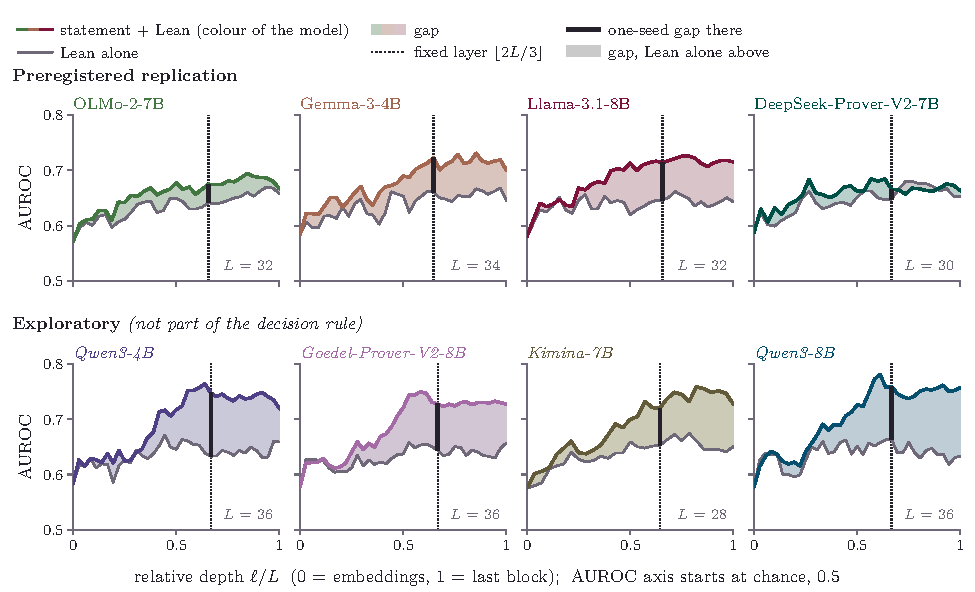
\includegraphics[width=\linewidth]{figuras_v3/curvas_por_modelo.pdf}
\caption{Layer by layer. AUROC of a linear probe reading the statement with the Lean code (each model in its own colour) and the Lean code alone (grey) on the 450 CriticLeanBench formalizations, mean over the Lean tokens; the shaded area is their gap, grey where the Lean code alone is above. The dotted line marks the layer fixed in advance for readout~(ii), $\lfloor 2L/3 \rfloor$, and the black segment is a one-seed version of the gap that readout measures. Top row: the preregistered replication. Bottom row: exploratory models. Descriptive: one seed, no layer selection, no intervals; nothing in the paper is decided from this figure.}
\label{fig:relieve}
\end{figure}


\paragraph{Data.}
Level~A uses the 450 CriticLeanBench formalizations that compile \citep{criticlean}, of which 250 are faithful and
200 unfaithful. Their labels were proposed by a model and validated by human reviewers.

\paragraph{Discovery.}
The effect was first seen in a single model. The first run was on Qwen3-4B, at the last token, with nested layer
selection and 100 permutations. It gave
$\D$ = +0.088 \ic{0.039}{0.134} with permutation $p = 0.0099$, the smallest value 100 permutations can return. Two
Lean-trained models, Goedel-Prover-V2 and Kimina, were run next under the same early rule. Their bootstrap intervals
excluded zero, but the permutation $p$-values of the difference were 0.16 and 0.25. That disagreement led to the
stricter rule below, the third version written that day. These runs carry no confirmatory weight.

Recomputed under the preregistered pipeline, the three discovery models give +0.091, +0.043 and +0.044 under
readout~(i), and +0.095, +0.066 and +0.051 under readout~(ii). The statement alone already predicts the label,
since \vr{nl\_only} reaches 0.61 to 0.74 in the four replication models. For that reason every gap is also compared
with a stacked control.

\paragraph{Preregistration.}
The preregistration was signed on 4 November 2026 at 22:29 (UTC$-$5), before any of the four new models was run.
Under its rule, a model passes if two conditions hold in either readout. Condition~(a) is that its $p$-value from
1000 permutations is below 0.05 after Holm correction \citep{holm} over the eight tests (four models, two
readouts). Each permutation shuffles the labels, refits both probes and recomputes $\D$. Condition~(b) is that the
interval of \vr{full} minus stacked lies entirely above zero. The global claim holds if at least three of four
models pass and the random-effects interval lies above zero in the same readout.

Two clauses of this rule were confirmed by the first author on 5 November, after the results of readout~(ii) had
been seen. One is that a model may pass with either readout, and the other is that the global claim is read within a
single readout. Neither changes a numerical threshold, though the first settles whether a model must pass in one
readout or in both, and we record them as a deviation.
Both clauses were already in the document signed on 4 November.

The permutation test and the bootstrap interval answer different questions. The first refits the probes under
shuffled labels, whereas the second resamples groups with the fitted scores held fixed. That is why
Table~\ref{tab:a} can show an interval clear of zero beside $p = 0.040$.

\begin{table}[h]
\centering
\caption{Level A, preregistered models. With eight tests the smallest raw $p$ must fall below 0.00625 to survive
Holm; the smallest observed is 0.040 (0.32 after adjustment). Two permutation tests of readout~(i) were not run because condition~(b)
already failed there and they could not change the decision.}
\label{tab:a}
\vspace{2pt}
{\small\setlength{\tabcolsep}{4pt}
\begin{tabular}{@{}lccccc@{}}
\toprule
 & \vr{full} & \vr{lean\_only} & $\D$ [95\% CI] & \vr{full} $-$ stacked [95\% CI] & $p$ (raw)\\
\midrule
\multicolumn{6}{@{}l}{\emph{Readout (ii): mean over Lean tokens, fixed layer}}\\
OLMo-2-7B             & 0.724 & 0.679 & +0.044 [+0.009, +0.079] & +0.049 [+0.014, +0.083] & 0.084\\
Gemma-3-4B            & 0.745 & 0.688 & +0.058 [+0.021, +0.094] & +0.067 [+0.030, +0.102] & 0.040\\
Llama-3.1-8B          & 0.736 & 0.682 & +0.054 [+0.018, +0.088] & +0.056 [+0.021, +0.089] & 0.040\\
DeepSeek-Prover-V2-7B & 0.704 & 0.678 & +0.025 [−0.008, +0.061] & +0.033 [−0.001, +0.067] & 0.191\\
\midrule
\multicolumn{6}{@{}l}{\emph{Readout (i): last token, layer by nested cross-validation}}\\
OLMo-2-7B             & 0.738 & 0.705 & +0.032 [−0.011, +0.075] & +0.032 [−0.007, +0.069] & 0.195\\
Gemma-3-4B            & 0.726 & 0.688 & +0.038 [−0.009, +0.085] & +0.013 [−0.029, +0.055] & not run\\
Llama-3.1-8B          & 0.712 & 0.723 & −0.011 [−0.056, +0.031] & −0.059 [−0.098, −0.021] & not run\\
DeepSeek-Prover-V2-7B & 0.684 & 0.627 & +0.056 [+0.008, +0.104] & +0.043 [+0.003, +0.085] & 0.084\\
\bottomrule
\end{tabular}}
\end{table}

\paragraph{Decision.}
No model passes. Under readout~(ii) the interval of \vr{full} minus stacked excludes zero in three of the four
models, so condition~(b) is largely met.
At that readout, however, the stacked control does not reach \vr{lean\_only} on its own. Its AUROC is 0.675, 0.678,
0.680 and 0.670 in the order of Table~\ref{tab:a}, against 0.679, 0.688, 0.682 and 0.678. The stacker is a logistic
regression on the inner out-of-fold scores of the two probes, and there \vr{nl\_only} is read as the mean over the
statement tokens at the same fixed layer (0.660, 0.643, 0.673 and 0.650). Condition~(b) is therefore no stricter than
a positive gap at readout~(ii). No model, however, survives the multiplicity-corrected permutation test.
Under readout~(i) only DeepSeek-Prover-V2 meets condition~(b), with $p = 0.084$. The pre-specified sensitivity
analysis drops the 44 rows whose labels we had marked as doubtful, which leaves 406 rows. It leaves readout~(ii)
unchanged, with gaps of +0.046 \ic{0.010}{0.082}, +0.060 \ic{0.025}{0.096}, +0.060 \ic{0.023}{0.095} and +0.030
\ic{−0.006}{0.065} in the order of Table~\ref{tab:a}.

\paragraph{Meta-analysis.}
The preregistered DerSimonian--Laird estimate \citep{dl} over the four new models is +0.045 \ic{0.027}{0.062} under
readout~(ii), with $\tau^2 = 0$ and $I^2 = 0\%$. Under readout~(i) it is +0.028 \ic{−0.000}{0.056} ($I^2 = 34\%$).
Adding the three discovery models gives +0.056 \ic{0.041}{0.071} under~(ii) ($I^2 = 25\%$), but that figure is
exploratory, because it includes the model on which the effect was found.

The random-effects interval is too narrow, because the four models were scored on the same 450 formalizations and
their estimates are not independent. A post hoc bootstrap addresses this by resampling the same groups jointly for
the four models, with 2000 resamples stratified by class. It puts their mean gap at +0.045 \ic{0.021}{0.069}
under~(ii) and +0.029 \ic{−0.000}{0.058} under~(i). Its estimand is the mean gap of these four models over the
population of items, with the models held fixed, so it says nothing about a fifth model.

\begin{figure}[t]
\centering
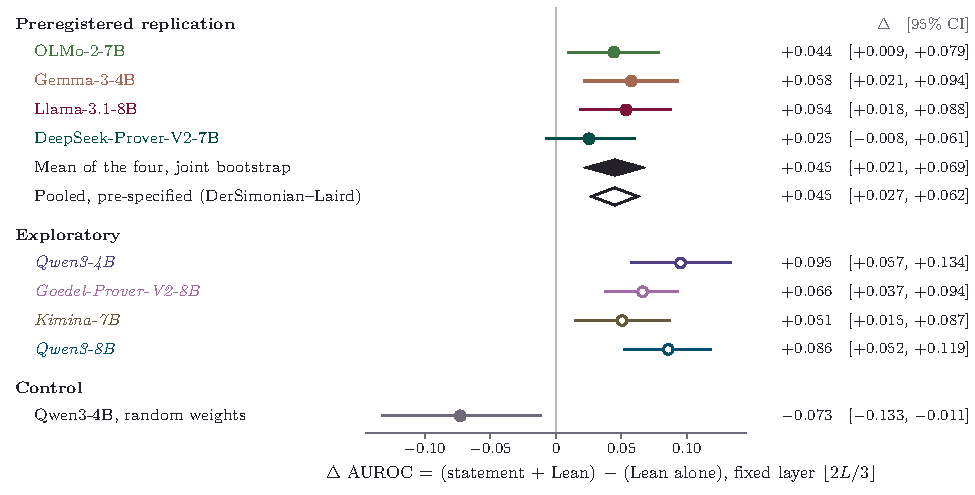
\includegraphics[width=\linewidth]{figuras_v3/forest_nivel_a.pdf}
\caption{Level A, readout (ii). Filled points: the four preregistered models. Filled diamond: their mean, with the post hoc joint bootstrap over items; outlined diamond: the preregistered DerSimonian--Laird estimate. Open points: exploratory models. Grey: the same architecture with random weights. Each model keeps its colour in every figure.}
\label{fig:forest}
\end{figure}

\paragraph{Null controls.}
Two null controls check whether the architecture alone, or a generic encoder, would produce the gap.
With random weights Qwen3-4B gives +0.008 \ic{−0.041}{0.056} under~(i) and −0.073 \ic{−0.133}{−0.011} under~(ii).
On bge-m3 sentence embeddings \citep{bgem3} the gap is −0.098 \ic{−0.153}{−0.044}. Neither produces a positive gap. Under readout~(ii) with random weights and on the embeddings the gap is
negative, with intervals below zero.

\paragraph{A later exploratory model.}
Qwen3-8B was added later and is exploratory. It gives +0.043 \ic{−0.004}{0.088} under~(i) and +0.086
\ic{0.052}{0.119} under~(ii), with \vr{full} minus stacked at +0.113 \ic{0.078}{0.148} under~(ii). No permutations
were run.

\paragraph{Source of the problem.}
CriticLeanBench draws its problems from twelve sources, and the proportion of faithful formalizations differs
between them. As a result, the source alone separates the labels with AUROC 0.578 \ic{0.525}{0.629}. A post hoc
analysis, run under readout~(ii) only, asks whether the gap is the source read by another route. One source, AIME,
has no faithful items (0 of 3) and contributes nothing.

The first check compares faithful and unfaithful formalizations only within the same source and pools the
comparison over sources. The mean gap of the four preregistered models under readout~(ii) is then +0.049
\ic{0.021}{0.079}. Model by model, this within-source gap is +0.052 \ic{0.006}{0.097} in OLMo-2, +0.081
\ic{0.035}{0.127} in Gemma-3, +0.052 \ic{0.009}{0.096} in Llama-3.1 and +0.013 \ic{−0.027}{0.053} in
DeepSeek-Prover-V2.

The second check trains the probe on eleven sources and tests it on the twelfth. It gives a gap of +0.079
\ic{0.031}{0.130} in OLMo-2, +0.091 \ic{0.039}{0.141} in Gemma-3, +0.104 \ic{0.054}{0.155} in Llama-3.1 and +0.043
\ic{−0.002}{0.088} in DeepSeek-Prover-V2. Held-out scores are compared only within their own source, at the fixed
layer, with one fit per source. These gaps are larger than those of Table~\ref{tab:a} because \vr{lean\_only} loses
more than \vr{full} when the source is held out. In Llama-3.1, for example, \vr{lean\_only} falls from 0.659 within
source to 0.596, while \vr{full} goes from 0.710 to 0.700. The Lean-only probe leans on features specific to each
source.

\paragraph{Where the separation is readable.}
Figure~\ref{fig:escaner} applies each layer's probe direction, fitted without the row in question, to the tokens at
each position of the prompt. The analysis is in the spirit of information-based (searchlight) mapping
\citep{searchlight}, with one difference. Instead of fitting a classifier at each position, we apply a single
direction, fitted on the mean over Lean tokens, position by position. Maps over layers and token positions are a
standard device in interpretability, usually built from causal interventions \citep{meng2022rome,geometry} or from
reading directions \citep{zou2023repe}. Ours shows where the label is linearly readable. It does not show where the
label is computed or whether the model uses it. Since it re-reads the data of readout~(ii), it is not an
independent test either.

In the five general-purpose models this direction, fitted on Lean tokens, is at or near chance over the statement
span, where the model has not yet read the Lean code. On average it lies between 0.49 and 0.52 there, and the one
exception is Qwen3-8B, at 0.521 \ic{0.501}{0.543}. It then rises over the Lean tokens in the upper layers. That
does not mean the statement carries no information about the label, since \vr{nl\_only} probes reach 0.61 to 0.74 in the four replication models.

Over the Lean tokens, the separation is weaker in four of the five models when the statement is removed. Averaged over those tokens in
the upper 60\% of the layers, the cell-wise AUROC with the statement exceeds the one without it by +0.043
\ic{0.032}{0.054} in Qwen3-8B, +0.039 \ic{0.028}{0.050} in Qwen3-4B, +0.031 \ic{0.019}{0.043} in Llama-3.1, +0.024
\ic{0.014}{0.035} in Gemma-3 and +0.012 \ic{−0.001}{0.024} in OLMo-2. The intervals come from 300 resamples of rows
with the directions held fixed. Under a paired null that swaps the two conditions within each row, with 500 swaps,
the 95th percentile of that difference is at most 0.011. That null gives $p = 0.002$ in four models, the smallest
value 500 swaps can return, and $p = 0.022$ in OLMo-2. In OLMo-2 the two procedures disagree, since its interval
includes zero, and we treat the difference in that model as not established. The region, moreover, was chosen after
seeing the maps, and the direction was fitted on the mean over Lean tokens and applied token by token. The maps are
exploratory.

\paragraph{Reading.}
The effect as preregistered, model by model, was not confirmed. With 450 rows per model, the instrument does not
resolve a gap of this size after correction. The post hoc joint bootstrap puts the mean gap of the four new models
at +0.045 \ic{0.021}{0.069} under the fixed-layer readout and +0.029 \ic{−0.000}{0.058} under the last-token
readout, and neither null control shows a positive gap. This is not a replication under the rule we wrote.
Figure~\ref{fig:relieve} shows the same data layer by layer.

\begin{figure}[p]
\centering
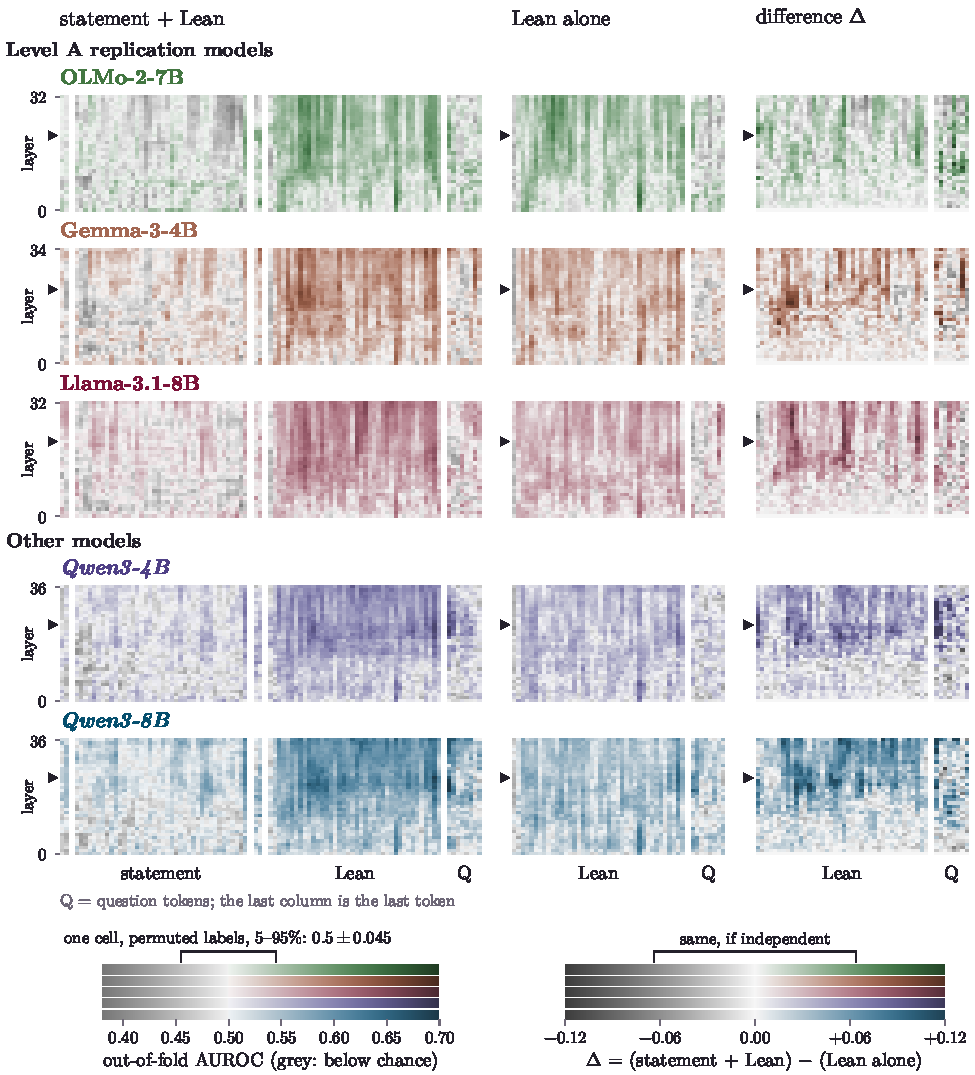
\includegraphics[width=\linewidth]{figuras_v5/escaner2d_modelos_v5.pdf}
\caption{Where in the prompt and at which depth the separation is readable, in the five general-purpose models. Each cell is the out-of-fold AUROC of the layer's probe direction applied to the tokens at that position, on the 450 CriticLeanBench formalizations; spans are stretched to a fixed width and cells are raw. Left: the prompt with statement and Lean. Middle: the Lean code alone. Right: their difference, in the model's colour where the statement adds and in grey where it subtracts. All models share one lightness scale, so equal values are equally dark; cells below chance are grey. The brackets on the keys give the size of single-cell noise by a normal approximation, and for the difference an independence bound. The marker is the layer $\lfloor 2L/3 \rfloor$. Exploratory: one seed, a direction fitted on the mean over Lean tokens and applied token by token.}
\label{fig:escaner}
\end{figure}

% ------------------------------------------------------------------ 5
\section{Level B: minimal pairs certified by Lean}

\paragraph{Construction.}
Each pair holds two minimal edits of the same original Lean statement. Lean certifies one of them as equivalent to
the original, and that edit is the faithful member. Lean certifies the other as not equivalent, and it is the
unfaithful member. The natural-language statement is identical in both, so the statement alone cannot separate
them. The \vr{nl\_only} probe accordingly gives 0.500 by construction, which serves as a check of the pipeline.

Certification compares each edit with its original and never tries to prove the theorem. A faithful edit is certified
when Lean proves that the edited hypothesis or conclusion is equivalent to the original one, with structural tactics
only. An unfaithful edit is certified by a witness, that is, concrete values that separate the two formulas and that
Lean checks. Witnesses are searched only when every variable involved is a natural, integer, rational or real number.

Unfaithful edits fall into three families. Family A makes the theorem stronger, B makes it weaker, and C turns it
into a different theorem. Within C, C2 changes a numeral and C3 changes something else.
Table~\ref{tab:bejemplos} shows one pair from each.

\begin{table}[h]
\centering
\caption{Level B, one pair per family of edit, chosen by a fixed rule: the pair with the fewest edited tokens in its two members and, among ties, the first in the index. Only the edited fragment of each Lean statement is shown. The unfaithful member carries the faithful edit as well. The statement of the C2 pair is cut after its first sentence.}
\label{tab:bejemplos}
\vspace{2pt}
{\footnotesize
\begin{tabularx}{\linewidth}{@{}lX>{\raggedright\arraybackslash}p{0.2\linewidth}>{\raggedright\arraybackslash}p{0.2\linewidth}>{\raggedright\arraybackslash}p{0.2\linewidth}@{}}
\toprule
 & Statement & Original & Faithful edit & Unfaithful edit\\
\midrule
A & Let \(k\) be a given positive integer with \(k\geqslant2\). Prove that the product of three consecutive positive integers cannot be the \(k\) -th power of an integer. & \texttt{2 $\le$ k} & \texttt{1 $<$ k} & \texttt{1 $\le$ k}\\
\addlinespace
B & Let $n$ be a fixed positive integer. Determine the smallest possible rank of an $n \times n$ matrix that has zeros along the main diagonal and strictly positive real numbers off the main diagonal. Prove that the answer is: 3 & \texttt{0 $<$ n} & \texttt{1 $\le$ n} & \texttt{1 $<$ n}\\
\addlinespace
C2 & The generic rank of a $4 \times m \times m$ tensor is $\lceil 4m^2 / (2m + 2) \rceil$ [\ldots] & \texttt{3 $\le$ m} & \texttt{2 $<$ m} & \texttt{3 $<$ m}\\
\addlinespace
C3 & The trivial upper bound, by counting pairs of points: for $k \geq 2$, $f_k(n) \cdot k(k-1) \leq n(n-1).$ & \texttt{2 $\le$ k} \newline \texttt{numLinesWithPointsMax k n * (k * (k - 1)) $\le$ n * (n - 1)} & \texttt{1 $<$ k} \newline \texttt{numLinesWithPointsMax k n * (k * (k - 1)) $\le$ n * (n - 1)} & \texttt{1 $<$ k} \newline \texttt{numLinesWithPointsMax k n * (k * (k - 1)) $\ge$ n * (n - 1)}\\
\bottomrule
\end{tabularx}}
\end{table}

Origins come from formal-conjectures \citep{fc,fcpaper} (323 pairs) and
FormalMATH-Lite \citep{formalmath} (54 pairs). After exclusions fixed before any activation was extracted, the main
batch has 377 pairs from 256 origins in 189 source files, certified with Lean~4.34.1 \citep{lean4,mathlib}.
Lean certified 408 pairs. A review by a language model, not by a human, then removed 31 pairs. In 9 the original was itself not faithful to its
statement. In 23, all of family~A, the witness separates the formulas but the edit only adds a case in which the
conclusion holds trivially, so the two statements say the same. One pair is in both groups. For
comparison, on all 408 the gap in Qwen3-4B is +0.213 \ic{0.150}{0.280}.

The batch falls short of the 400 pairs and 300 origins the rule asked for, which is what ``reduced power'' means in
Table~\ref{tab:b}. Under the same rule, a model whose interval for $\D$ includes zero is recorded as a null with its
upper bound. The rule also allows the phrase ``beyond the surface'' only when the interval of \vr{full} minus
cross-surface lies above zero. The test first planned for this level used triplets. No certifiable batch of
triplets could be built, and the pairs were declared a development batch.
A surface check fixed in advance also failed. On the 408 certified pairs, a logistic regression on unigrams and
bigrams of the Lean code alone reaches a paired AUROC of 0.706, an excess of 0.081 over an unsupervised baseline, against a
limit of 0.05.

Folds are grouped by source file, whereas the paired AUROC and the bootstrap take the origin as their unit. With the
189 source files as the unit instead, the gap is +0.229 \ic{0.157}{0.301}, +0.109 \ic{0.046}{0.174}, +0.086
\ic{0.019}{0.158} and +0.037 \ic{−0.038}{0.106}, in the order of Table~\ref{tab:b}.

\begin{table}[h]
\centering
\caption{Level B, 377 pairs. Top: the central test, paired AUROC at the last token. With 100 within-pair permutations the
smallest attainable $p$ is 0.0099; the permutation test uses the statistic of seed 0 (0.250, 0.118, 0.104 and 0.079), while the $\D$ column is the five-seed estimate. The rule decides on the interval of the five-seed estimate. The permutation $p$ is reported beside it. Once corrected across the four models by Holm's method, only that of Qwen3-4B stays below 0.05, at 0.040; the other three rise to 0.059. By the rule, the first three rows are positive at reduced power and the fourth is
a null with upper bound 0.107.}
\label{tab:b}
\vspace{2pt}
\begin{tabular}{@{}lcccc@{}}
\toprule
 & \vr{full} & \vr{lean\_only} & $\D$ [95\% CI] & $p$ ($\D$)\\
\midrule
Qwen3-4B     & 0.807 & 0.582 & +0.225 [+0.158, +0.291] & 0.0099\\
OLMo-2-7B    & 0.766 & 0.664 & +0.102 [+0.039, +0.164] & 0.0198\\
Llama-3.1-8B & 0.762 & 0.678 & +0.084 [+0.023, +0.146] & 0.0198\\
Gemma-3-4B   & 0.684 & 0.643 & +0.041 [−0.023, +0.107] & 0.0594\\
\midrule
\multicolumn{5}{@{}l}{\emph{Second readout: mean over Lean tokens (no permutation test run)}}\\
Qwen3-4B     & 0.944 & 0.780 & +0.164 [+0.120, +0.210] & ---\\
OLMo-2-7B    & 0.859 & 0.775 & +0.084 [+0.039, +0.129] & ---\\
Llama-3.1-8B & 0.902 & 0.768 & +0.135 [+0.090, +0.180] & ---\\
Gemma-3-4B   & 0.895 & 0.777 & +0.117 [+0.072, +0.162] & ---\\
\bottomrule
\end{tabular}
\end{table}

\begin{table}[h]
\centering
\caption{Level B controls, all at the last token. The n-gram and cross-surface classifiers reach 0.729 and 0.688 on their own. The last column repeats the central test on the 309 pairs that remain when the numeral
edits (C2) are removed.}
\label{tab:bcontroles}
\vspace{2pt}
{\footnotesize\setlength{\tabcolsep}{3pt}
\begin{tabular}{@{}lcccc@{}}
\toprule
\vr{full} minus & n-grams & cross-surface & P(Yes) & without C2, vs.\ \vr{lean\_only}\\
\midrule
Qwen3-4B     & +0.078 [+0.010, +0.141] & +0.118 [+0.058, +0.177] & −0.032 [−0.074, +0.008] & +0.187 [+0.112, +0.260]\\
OLMo-2-7B    & +0.037 [−0.023, +0.094] & +0.077 [+0.018, +0.135] & +0.040 [−0.010, +0.091] & +0.073 [+0.006, +0.139]\\
Llama-3.1-8B & +0.033 [−0.035, +0.098] & +0.073 [+0.012, +0.133] & +0.033 [−0.022, +0.085] & +0.019 [−0.049, +0.088]\\
Gemma-3-4B   & −0.045 [−0.107, +0.018] & −0.005 [−0.066, +0.060] & +0.124 [+0.062, +0.189] & +0.002 [−0.071, +0.077]\\
\bottomrule
\end{tabular}}
\end{table}

\paragraph{What the controls say.}
The first control replaces the statement with the wrong one. With it the probe falls to chance in every model
(0.506 to 0.537), so the gain needs the \emph{right} statement. Against the cross-surface control, three models
keep a positive margin and Gemma-3 does not. On this batch, however, plain n-grams of the two
texts separate the pairs better (0.729) than the cross-surface features do (0.688), so they are the harder control
overall. Against them only Qwen3-4B keeps a margin (+0.078 \ic{0.010}{0.141}), and in the other three the interval
includes zero. On the numeral edits examined below, in contrast, the cross-surface features reach 0.933, which the
n-grams do not.

The model's own answer sets a further limit. In Qwen3-4B its yes/no answer separates the pairs as well as the probe
(0.839 against 0.807), so there the probe adds nothing detectable over that answer. At the last token, no model
exceeds both the n-gram control and its own P(Yes) with intervals above zero. A further control, also in Qwen3-4B,
scores the unedited original against its faithful edit and finds them indistinguishable (0.520), which rules out
``having been edited'' as the signal.

\paragraph{The second readout.}
The controls above were computed against the last-token probe. The gap over the Lean code alone was measured at both, and it also depends on the readout. At the mean over
Lean tokens it is positive in all four models, at +0.164 \ic{0.120}{0.210} in Qwen3-4B, +0.084 \ic{0.039}{0.129} in
OLMo-2, +0.135 \ic{0.090}{0.180} in Llama-3.1 and +0.117 \ic{0.072}{0.162} in Gemma-3. The null in Gemma-3 is
therefore specific to the last token.

At that readout, however, \vr{lean\_only} is itself much higher (0.77 to 0.78), so the Lean code alone gives away more
than Table~\ref{tab:b} suggests. A Lean-only probe at 0.78 on pairs that share one statement is above the n-gram
baseline of both texts (0.729). The n-grams therefore do not capture all that the Lean text reveals about which
edit is the unfaithful one. No permutation test was run on this readout.

\paragraph{Controls at the second readout.} After the analyses above we computed the same controls for the second
readout, under a rule written before running them. The analysis is exploratory and post hoc. At the mean over Lean
tokens, \vr{full} exceeds the n-gram control, the cross-surface control and the model's own P(Yes) in all four models,
with every interval above zero (Table~\ref{tab:bcontroles2}). Over P(Yes) the margin is +0.105 \ic{0.070}{0.142} in
Qwen3-4B, +0.134 \ic{0.086}{0.187} in OLMo-2, +0.174 \ic{0.129}{0.218} in Llama-3.1 and +0.335 \ic{0.275}{0.392} in
Gemma-3.

We also trained a single classifier on the n-gram and cross-surface features together. On its own it reaches 0.787,
and \vr{full} at the second readout stays above it in the four models; the smallest margin is +0.072
\ic{0.023}{0.123}, in OLMo-2. At the last token, in contrast, \vr{full} cannot be told apart from this combined
control in three models, and in Gemma-3 the control is ahead (−0.104 \ic{−0.164}{−0.045}). The second-readout margins
hold on the 309 pairs without the numeral edits.

\begin{table}[h]
\centering
\caption{Level B controls at the second readout (mean over Lean tokens), 377 pairs. The n-gram, cross-surface and combined classifiers reach 0.729, 0.688 and 0.787 on their own. Exploratory and post hoc.}
\label{tab:bcontroles2}
\vspace{2pt}
{\footnotesize\setlength{\tabcolsep}{2pt}
\begin{tabular}{@{}lccccc@{}}
\toprule
\vr{full} minus & AUROC & n-grams & cross-surface & P(Yes) & combined\\
\midrule
Qwen3-4B     & 0.944 & +0.216 [+0.166, +0.266] & +0.256 [+0.204, +0.310] & +0.105 [+0.070, +0.142] & +0.157 [+0.111, +0.203]\\
OLMo-2-7B    & 0.859 & +0.131 [+0.082, +0.182] & +0.171 [+0.114, +0.229] & +0.134 [+0.086, +0.187] & +0.072 [+0.023, +0.123]\\
Llama-3.1-8B & 0.902 & +0.174 [+0.123, +0.227] & +0.214 [+0.159, +0.266] & +0.174 [+0.129, +0.218] & +0.115 [+0.068, +0.164]\\
Gemma-3-4B   & 0.895 & +0.166 [+0.113, +0.215] & +0.206 [+0.154, +0.259] & +0.335 [+0.275, +0.392] & +0.107 [+0.061, +0.152]\\
\bottomrule
\end{tabular}}
\end{table}

\paragraph{Shifting the mean along the separating axis.} A decodable label need not be used \citep{elazar2021amnesic}.
We therefore intervened, first in Qwen3-4B as an exploratory analysis and then in the other three models under a rule
fixed before running them. At every layer but the last we take the difference between the class means of the second
readout, estimated out of fold. We then shift all Lean tokens along that direction, so that their mean coordinate
travels toward the opposite class by the full distance between the class means, and we read P(Yes). The control
applies the same shift along 20 random directions. A model meets the criterion if the drop in the paired AUROC of
P(Yes) exceeds the mean random drop with a 95\% interval above zero, and also exceeds each of the 20 random drops. The
class means are estimated on the training rows of five folds grouped by source file. The sign of the shift comes from
the label of each row, so the intervention uses the labels of the rows it is evaluated on. The hooks act on the
embeddings and on the output of every block but the last, in the same forward pass. The target is set layer by layer,
so the shift does not accumulate. The random directions are Gaussian vectors scaled to unit length, drawn separately
for each layer, and they receive a shift of the same size and sign. P(Yes) is the probability of Yes divided by that
of Yes plus No, and the intervals resample the 256 origins. Adding a difference of means to the activations is the
basis of contrastive activation addition \citep{rimsky2024steering}, and the comparison with random directions follows
the control of \citet{elazar2021amnesic}.

Qwen3-4B meets the criterion. The AUROC of P(Yes) falls from 0.838 to 0.688, a drop of +0.145 \ic{0.112}{0.177} over the random
mean, and no random direction reaches it. That run was designed after an earlier null, described below, so it is post
hoc. Of the three models tested under the rule fixed in advance, OLMo-2 meets the criterion (0.717 to 0.432; +0.270
\ic{0.233}{0.309}), and Llama-3.1 and Gemma-3 do not. In both, the drop exceeds the random mean (+0.102
\ic{0.072}{0.132} and +0.115 \ic{0.077}{0.153}), but 2 and 6 of the 20 random directions lower the AUROC as much or
more. In Gemma-3 the model's own P(Yes) barely separates the pairs to begin with (0.590), and the rule had flagged
that case in advance. In Llama-3.1 the direction built from \vr{lean\_only} moves the answer as much as the one built
from \vr{full} (difference +0.015 \ic{−0.029}{0.057}), so there the effect cannot be attributed to the statement.
In Gemma-3 the interval of the same difference also includes zero (+0.049 \ic{−0.003}{0.100}). The secondary analyses
are in Appendix~\ref{app:intervencion}.
A natural worry is that the shift only moves a surface feature, because the numeral edits can be told apart without
any model. The worry does not hold. When those pairs are set aside, the effect in Qwen3-4B and OLMo-2 is about the
same as before, and Llama-3.1 and Gemma-3 still fall short of the criterion (Appendix~\ref{app:intervencion}). The
directions were estimated with the numeral pairs among the training rows, however, so the result is narrower than it
sounds. It shows that the shift changes the answer on pairs that alter no numeral, and it leaves open how much of the
direction those pairs shaped. A
shift four times larger takes the AUROC below 0.5 in the four models (Table~\ref{tab:bintervencion} and
Figure~\ref{fig:bintervencion}).

An earlier intervention gave a null. In Qwen3-4B we fixed, on the Lean tokens and at every layer, the coordinate along
the logistic-probe direction of the fixed layer at its mean. P(Yes) did not change more than with a random direction
(−0.009 \ic{−0.026}{0.008}). That operation is a one-direction relative of linear concept erasure
\citep{ravfogel2020null,belrose2023leace}. The two interventions differ in the direction and in the operation, so the
null cannot be attributed to the direction alone. In a related setting, \citet{geometry} report that
difference-of-means directions are more causally implicated than those of logistic probes in most of their conditions,
in two LLaMA-2 models and with additive shifts.

\begin{figure}[!ht]
\centering
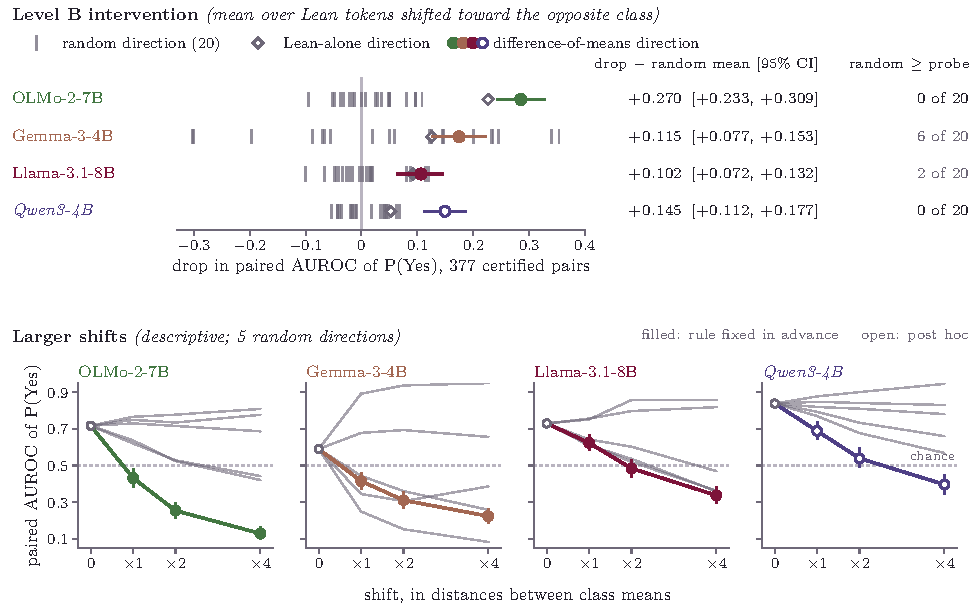
\includegraphics[width=\linewidth]{figuras_v5/intervencion_nivel_b.pdf}
\caption{Level B intervention. Top: drop in the paired AUROC of P(Yes) when the mean over Lean tokens is shifted toward the opposite class by the full distance between class means. Each grey tick is one of 20 random directions given the same shift, the diamond is the direction built from \vr{lean\_only}, and the coloured marker is the difference-of-means direction with its 95\% interval. The criterion asks for an interval above zero in the first column and for no tick at or to the right of the coloured marker. Bottom: paired AUROC of P(Yes) as the shift grows, for the difference-of-means direction (colour) and for five random directions (grey). Filled markers are models run under a rule fixed in advance; the open markers are Qwen3-4B, which is post hoc.}
\label{fig:bintervencion}
\end{figure}

\begin{table}[h]
\centering
\caption{Level B intervention, 377 pairs. Paired AUROC of P(Yes) with no intervention and after shifting the mean over Lean tokens toward the opposite class by the full distance between class means, along the difference-of-means direction at every layer but the last. ``Random'' is the same shift along 20 random directions (mean; maximum of the drop). The criterion asks for an interval above zero in the sixth column and for no random direction with an equal or larger drop. The last two columns give the AUROC after shifts two and four times larger. Qwen3-4B is post hoc; the other three models were run under a rule fixed in advance. The base was recomputed in the intervention run and differs from the stored P(Yes) of Table~\ref{tab:controlesnivel} (0.839, 0.726, 0.729, 0.560) by up to 0.030, in Gemma-3.}
\label{tab:bintervencion}
\vspace{2pt}
{\footnotesize\setlength{\tabcolsep}{3pt}
\resizebox{\linewidth}{!}{\begin{tabular}{@{}lcccccccc@{}}
\toprule
 & base & shifted & drop & random & drop minus random mean & random $\geq$ probe & $\times 2$ & $\times 4$\\
\midrule
Qwen3-4B     & 0.838 & 0.688 & +0.149 [+0.110, +0.188] & +0.005; +0.068 & +0.145 [+0.112, +0.177] & 0 of 20 & 0.539 & 0.396\\
OLMo-2-7B    & 0.717 & 0.432 & +0.285 [+0.242, +0.330] & +0.015; +0.108 & +0.270 [+0.233, +0.309] & 0 of 20 & 0.254 & 0.129\\
Llama-3.1-8B & 0.729 & 0.623 & +0.106 [+0.063, +0.147] & +0.004; +0.120 & +0.102 [+0.072, +0.132] & 2 of 20 & 0.484 & 0.337\\
Gemma-3-4B   & 0.590 & 0.415 & +0.175 [+0.125, +0.225] & +0.060; +0.354 & +0.115 [+0.077, +0.153] & 6 of 20 & 0.311 & 0.224\\
\bottomrule
\end{tabular}}}
\end{table}

\paragraph{The effect concentrates in family C, and in Qwen3-4B the numeral edits inside C are a surface effect.}
Against the Lean code alone, family C gives the largest gap in all four models (Table~\ref{tab:bfam}). In families A and
B the interval excludes zero only in Qwen3-4B and, for family A, in OLMo-2, while Llama-3.1 and Gemma-3 stay within
0.023 of zero. A post hoc split in Qwen3-4B (Figure~\ref{fig:b}, bottom) shows why. In C2 the cross-surface
control reaches 0.933 on its own, which is indistinguishable from the activations at 0.913 (difference −0.020
\ic{−0.103}{0.056}). This happens because in 84\% of those pairs the unfaithful member has more Lean numerals
absent from the statement than the faithful one, and a feature that counts them needs no model. Against
the cross-surface control, families A and B are not distinguishable from zero (+0.082 \ic{−0.038}{0.195} and +0.098
\ic{0.000}{0.195}). C3 is clearly above it (+0.385 \ic{0.192}{0.577}), though on only 31 pairs. The split is
post hoc, on one model, and without correction for multiplicity.


\begin{table}[h]
\centering
\caption{Level B by family of edit: gap over the Lean code alone at the last token, with 95\% intervals. Descriptive, not part of the decision.}
\label{tab:bfam}
\vspace{2pt}
{\small
\begin{tabular}{@{}lccc@{}}
\toprule
 & A: stronger (142 pairs) & B: weaker (136) & C: other theorem (99)\\
\midrule
Qwen3-4B     & +0.141 [+0.038, +0.248] & +0.129 [+0.027, +0.230] & +0.427 [+0.320, +0.539]\\
OLMo-2-7B    & +0.103 [+0.015, +0.191] & +0.039 [−0.055, +0.133] & +0.230 [+0.129, +0.331]\\
Llama-3.1-8B & +0.023 [−0.080, +0.126] & −0.023 [−0.117, +0.074] & +0.337 [+0.236, +0.444]\\
Gemma-3-4B   & −0.008 [−0.126, +0.107] & −0.023 [−0.121, +0.074] & +0.213 [+0.090, +0.337]\\
\bottomrule
\end{tabular}}
\end{table}

\paragraph{Without C2.}
When the numeral edits are removed and the central test is repeated (Table~\ref{tab:bcontroles}, last column), the
gap over the Lean code alone remains in Qwen3-4B and, narrowly, in OLMo-2, and vanishes in Llama-3.1 and Gemma-3. We exclude C2
from the primary population of the confirmatory protocol.

\begin{figure}[t]
\centering
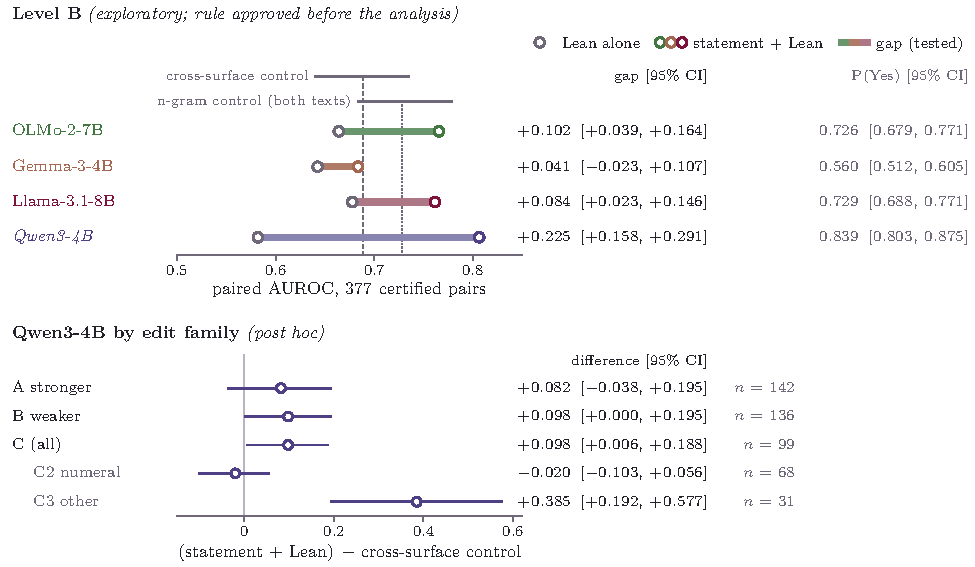
\includegraphics[width=\linewidth]{figuras_v3/nivel_b.pdf}
\caption{Level B. Top: paired AUROC of the probe reading the Lean code alone (grey) and the statement with the Lean code (model colour); the bar between them is the tested gap, with its interval in the first column and the model's own P(Yes) in the second. The dashed and dotted lines are the cross-surface and n-gram controls, with their intervals above. Bottom: \vr{full} minus cross-surface in Qwen3-4B by family of edit (post hoc).}
\label{fig:b}
\end{figure}

% ------------------------------------------------------------------ 6
\section{Level C: ProofNetVerif and transfer}

\paragraph{Data.}
ProofNetVerif \citep{proofnetverif} contains 3752 pairs of statement and Lean formalization, 1142 of them labelled
faithful. By our count the pairs fall into 361 statements, 217 of which have both faithful and unfaithful formalizations.
Folds and bootstrap are grouped by statement, so the effective sample is 361 groups.

\begin{table}[h]
\centering
\caption{Level C. Qwen3-4B was run under the approved rule and is reportable under it; Llama-3.1-8B was run
afterwards and is exploratory. A sanity permutation test of each AUROC, with 20 permutations, returned its minimum, $p = 0.048$, in
both models. The transfer value for Llama-3.1-8B is at the selected layer, layer 9 of 32; see the text.}
\label{tab:c}
\vspace{2pt}
\begin{tabular}{@{}lcc@{}}
\toprule
 & Qwen3-4B & Llama-3.1-8B\\
\midrule
\vr{full}                               & 0.832 [0.807, 0.855] & 0.791 [0.766, 0.819]\\
\vr{lean\_only}                         & 0.678 & 0.664\\
$\D$                                    & +0.154 [+0.121, +0.187] & +0.127 [+0.090, +0.165]\\
$\D$ within the same statement          & +0.177 [+0.141, +0.213] & +0.151 [+0.114, +0.195]\\
\vr{full} $-$ \vr{nl\_mismatched}       & +0.202 [+0.170, +0.234] & +0.175 [+0.138, +0.214]\\
\vr{full} $-$ P(Yes)                    & +0.044 [+0.020, +0.069] & +0.108 [+0.066, +0.150]\\
\vr{full} $-$ stacked                 & +0.146 [+0.115, +0.176] & +0.111 [+0.079, +0.145]\\
\vr{full} $-$ n-grams of both texts       & +0.144 [+0.105, +0.185] & +0.103 [+0.063, +0.148]\\
\midrule
Transfer from CriticLeanBench, $\D_T$   & +0.222 [+0.176, +0.267] & −0.017 [−0.064, +0.030]\\
\bottomrule
\end{tabular}
\end{table}

\paragraph{Result.}
The rule of this level calls the result positive if the interval of $\D$, from a bootstrap over statements, lies
entirely above zero. In both models the label is linearly decodable from the \vr{full} activations better than from the Lean code alone. The
gap persists within the same statement, where the statement can contribute neither difficulty nor source. In
Qwen3-4B it also survives surface n-grams of both texts (+0.144 \ic{0.105}{0.185}) and the stacked control
(+0.146 \ic{0.115}{0.176}). A second implementation, written without access to the first, gives $\D$ = +0.154 \ic{0.121}{0.187} in Qwen3-4B.

\paragraph{Transfer.}
A probe trained only on CriticLeanBench and applied unchanged to ProofNetVerif separates the pairs in Qwen3-4B
(\vr{full} 0.761, \vr{lean\_only} 0.539). In Llama-3.1-8B, at the layer selected on CriticLeanBench, it does not.
That layer is layer 9 of 32, the maximum of a nearly flat selection curve. There \vr{full} is 0.527 and
\vr{lean\_only}, at its own selected layer, is 0.544. In the same run the transfer values at later layers are
higher. They are 0.60 to 0.67 for \vr{full} from layer 11 upward, against at most 0.55 for \vr{lean\_only}. Those
values are post hoc and without intervals, and we draw no conclusion about transfer in this model.

Level~C is not restricted to formalizations that compile. Ill-typed candidates are therefore among its negatives,
which favours the Lean code-only probe.

% ------------------------------------------------------------------ 7
\section{What the three levels say together}

\begin{table}[h]
\centering
\caption{Status of the evidence. ``Model--readout pairs'' counts the signs of the eight preregistered estimates of Table~\ref{tab:a}.}
\label{tab:conjunta}
\vspace{2pt}
\begin{tabularx}{\linewidth}{@{}lXXX@{}}
\toprule
 & A: CriticLeanBench & B: certified pairs & C: ProofNetVerif\\
\midrule
Labels & human-validated & generator, certified by Lean & human, one annotator\\
Status & preregistered & exploratory & rule approved in advance (one model)\\
Sign of $\D$ & positive in 7 of 8 model--readout pairs & positive in 4 of 4 & positive in 2 of 2\\
Outcome under its rule & not confirmed per model; mean of the four +0.045 [0.021, 0.069] under (ii) and +0.029 [−0.000, 0.058] under (i), post hoc & at the last token, 3 positive at reduced power, 1 null & positive\\
Main threat & label noise and style & at the last token, n-grams of both texts, which only Qwen3-4B exceeds; surface in numeral edits; P(Yes) matches the probe in Qwen3-4B & contamination\\
\bottomrule
\end{tabularx}
\end{table}

The sign of the gap is the same in nearly every setting we examined. Reading the statement together with the Lean code
separates better than reading the Lean code alone. The levels differ, however, in how much each of them licenses.
Level~A is the only preregistered test, and it did not pass. Level~B has the cleanest design, with the statement
held fixed and the labels certified by Lean, but it is a development batch and part of its effect is surface.
In two of four models, one of them under a rule fixed in advance, a shift along the axis on which the second readout
separates the classes changes the answer more than the same shift along random directions. This does not show what the
model computes, and it does not hold in the other two. A shift can also change the output through a pathway other than
the one it targets \citep{makelov2024subspace}. At
Level~C the effect is large and, for Qwen3, the protection against memorisation is the weakest. No level alone
supports the claim that faithfulness is linearly decodable from frozen models beyond the Lean code alone.
Taken together, they justify asking the question again on data the models cannot have seen.

\begin{table}[h]
\centering
\caption{Controls by level. AUROC of the control on its own, or \vr{full} minus the control where marked with a sign. ``Not run'' means the control does not exist for that level.}
\label{tab:controlesnivel}
\vspace{2pt}
{\small
\begin{tabularx}{\linewidth}{@{}lXXX@{}}
\toprule
Control & A & B (last token) & C\\
\midrule
n-grams & Lean only: 0.682, level with \vr{lean\_only} (0.678 to 0.688) & both texts: 0.729 & \vr{full} minus: +0.144 Qwen3-4B, +0.103 Llama-3.1\\
Cross-surface & not run & 0.688 & not run\\
Stacked & Table~\ref{tab:a} & not applicable (\vr{nl\_only} is 0.500) & \vr{full} minus: +0.146, +0.111\\
\vr{nl\_mismatched} & not analysed & 0.506 to 0.537 & \vr{full} minus: +0.202, +0.175\\
P(Yes) & 0.47 to 0.51 in OLMo-2, Gemma-3 and Llama-3.1; 0.70 and 0.72 in Qwen3-4B and Qwen3-8B; not interpretable in DeepSeek-Prover-V2 & 0.839, 0.726, 0.729, 0.560 (order of Table~\ref{tab:b}) & 0.788 in Qwen3-4B\\
Random weights & Qwen3-4B only & not run & not run\\
bge-m3 & run & not run & not run\\
\bottomrule
\end{tabularx}}
\end{table}

% ------------------------------------------------------------------ 8
\section{Limitations}

\paragraph{Contamination.}
Part of the data was public before some of the models were released. ProofNetVerif was described in June 2024 and has been on Hugging Face
since February 2025, that is, before Qwen3 was released and around or after the release of Llama-3.1. At Level~B,
formal-conjectures became public in May 2025. By our dating, and with one known exception, the Lean statements of
the batch were not public before the release of the four models probed there. The exception is an origin whose
near-identical statement has been in Mathlib since July 2024. Earlier versions of the FormalMATH-Lite statements
were not checked. The natural-language statements, in contrast, are older in about 210 of the 256 origins, where
the problems were known and their formalizations were not.

\paragraph{Labels.}
The labels have a different weakness at each level. Level~A uses the benchmark's labels, proposed by a model and
validated by human reviewers, and some of them rest on broad criteria. Level~B labels come from the generator and
are certified by Lean. The screening that removed non-faithful originals, however, was done by a model, and one of
the sources of the batch, FormalMATH-Lite, has documented defects \citep{ammanamanchi2026faults}.
Level~C has a single annotator.

\begin{pendiente}
A blind human review of 80 items (40 from Level~B, 40 from Level~C), with agreement thresholds fixed in advance, is
in progress. Its agreement rates will be reported here and will bound the label noise of both levels.
\end{pendiente}

\paragraph{Power.}
The samples are 450 rows per model at Level~A, 256 origins at Level~B and 361 groups at Level~C.

\paragraph{Method.}
The probes are linear and their evidence is correlational. In Qwen3-4B at Level~B the model's own answer separates as
well as the probe. We intervened on one family of directions, at Level~B only. The intervention meets its criterion in two of four
models, and the run in Qwen3-4B is post hoc.
One control was not run. Directions built as differences of means from shuffled labels would show how much of the
effect comes from fitting a direction to these activations at all.

\paragraph{Decisions after the fact.}
Several analyses were decided after seeing results. They are the split of family C, the exclusion of C2, the runs
on Qwen3-8B and on Llama at Level~C, the three later models and the second readout at Level~B, the by-source
control, the joint bootstrap, the layer-by-layer figures, and the maps with their region statistics and swap null.
The controls at the second readout and the two interventions at Level~B came later still, between 11 and 13
November. They are labelled as such where they appear.

% ------------------------------------------------------------------ 9
\section{Conclusion}

Our question was whether a frozen model's activations separate a formalization that says what was meant from
one that does not, beyond what the formal text alone reveals. The answer the pilot supports is narrow. The gap is
positive in most settings we tried, a few points of AUROC at Level~A, and it is absent with random weights or
generic embeddings. Several of its intervals, however, include zero. They are most of those of the last-token
readout at Level~A, where Llama-3.1 is negative, and that of Gemma-3 at the last token at Level~B. Transfer in
Llama-3.1 at the selected layer is indistinguishable from zero. The gap did not pass the per-model test we
committed to in advance. On certified pairs part of it is a numeral that the statement lacks, and at Level~C the
data were public before one of the two models was released.

The pilot thus yields a small signal and a list of the ways in which it could be an artefact. The draft protocol in
Appendix~\ref{app:protocolo} is designed to remove or measure the surface, contamination and label items on that
list. It does not yet address a P(Yes) that matches the probe. The maps of Figure~\ref{fig:escaner} show where the
fixed-layer direction separates the classes. Whether the model uses that direction is a causal question, which
probing cannot answer and an intervention along the probe direction could.
At Level~B we ran such an intervention on a related direction, the difference of class means at each layer. It changes
the answer more than random directions do in two of four models, one of them in a post hoc run.

\paragraph{Use of AI tools.}
The analysis code and the first implementation of every level were written with AI coding assistants under rules
set by the first author. He approved each decision rule before its analysis ran, and the results will be compared
against an implementation he writes by hand before they are reported as findings. That comparison is pending. The
authors are responsible for all claims.

\paragraph{Code and data.}
The repository will be released with the preprint at \url{https://github.com/cmorregof}. It will contain the decision
rules with their hashes and times, the certified pairs, the cross-surface features, and every result file cited
here.


\bibliography{refs}
\bibliographystyle{tmlr}

\appendix
\section{Models and revisions}\label{app:modelos}
\begin{table}[h]
\centering
\caption{Models, pinned revisions, and number of residual-stream positions read (embeddings plus each block).}
\vspace{2pt}
\begin{tabular}{@{}llcc@{}}
\toprule
Model & Hugging Face identifier & Revision & Layers + emb.\\
\midrule
Qwen3-4B              & \vr{Qwen/Qwen3-4B}                         & \vr{1cfa9a72} & 37\\
Qwen3-8B              & \vr{Qwen/Qwen3-8B}                         & \vr{b968826d} & 37\\
OLMo-2-7B             & \vr{allenai/OLMo-2-1124-7B-Instruct}       & \vr{470b1fba} & 33\\
Gemma-3-4B            & \vr{google/gemma-3-4b-it}                  & \vr{093f9f38} & 35\\
Llama-3.1-8B          & \vr{meta-llama/Llama-3.1-8B-Instruct}      & \vr{0e9e39f2} & 33\\
DeepSeek-Prover-V2-7B & \vr{deepseek-ai/DeepSeek-Prover-V2-7B}     & \vr{a8d9e144} & 31\\
Goedel-Prover-V2-8B   & \vr{Goedel-LM/Goedel-Prover-V2-8B}         & \vr{dfd02e62} & 37\\
Kimina-7B             & \vr{AI-MO/Kimina-Autoformalizer-7B}        & \vr{ddd47cb4} & 29\\
\bottomrule
\end{tabular}
\end{table}

\section{Deviations and late decisions}\label{app:desviaciones}

The list below is taken from the reports of each level. The project log holds a longer numbered list, which will be
released with the repository, and nothing here replaces it.

\begin{description}[leftmargin=1.2em]
\item[4 Nov] Three versions of the Level~A rule were written in one day. The third, signed at 22:29, is the one
applied here. Goedel-Prover-V2 and Kimina had been run under the first and are reported as a failed first attempt.
\item[5 Nov, 08:37] An error in the permutation matrix of readout~(i) in the analysis script was corrected and
DeepSeek-Prover-V2 was rerun. Readout~(ii) was not affected.
\item[5 Nov] When the tokenizer's offsets do not line up with the text, extraction falls back to locating the Lean
tokens by prefix. This changed one model, DeepSeek-Prover-V2, in 1972 of its 2000 prompts.
The extraction covers the 500 rows of the benchmark in the four variants, and the analysis keeps the 450 that
compile.
\item[5 Nov] The first author confirmed two clauses of the Level~A document after the results of readout~(ii) had
been seen. One is that a model may pass with either readout, and the other is that the meta-analysis is read one
readout at a time. The remaining implementation clauses of that document were drafted by the coding assistant.
\item[5 Nov] For reasons of time, the permutations use an exact Newton solver in the basis of the singular value
decomposition in place of the library solver. The observed statistic is computed with the same solver.
\item[5--6 Nov] A restart of the machine lost the readout-(i) permutations of Gemma-3. On 6 November the first
author decided not to run them for Gemma-3 or Llama-3.1, because condition~(b) had already failed there. The
extraction of Llama-3.1 was resumed from saved state after a memory stall.
\item[6 Nov] At Level~B a surface check fixed in advance did not pass (0.706 on the certified pairs), and the
batch was declared exploratory. A code error in the control that scores the original against its faithful edit was
corrected (0.520). The split of family C by kind of edit was added the same day, after the results.
\item[7--8 Nov] Llama-3.1 at Level~C, Qwen3-8B at Level~A and three more models at Level~B were run after the
first results of each level.
\item[9 Nov] The by-source control, the joint bootstrap, the layer-by-position maps, their region statistics and
the swap null were added. The hypothesis of the draft protocol was changed to require both surface controls.
\item[11 Nov] The Level~B controls at the second readout, a check that the mean over Lean tokens does not depend on
the question, and the ablation of one direction in Qwen3-4B were run under a rule written and approved that day,
before running them. They are exploratory and post hoc.
\item[12 Nov] Under the same rule, the last-token gap was recomputed, as an exploratory analysis, on activations
extracted without the question. At Level~A the gap is not established without the question in any of the four models. The models are Qwen3-4B, OLMo-2, Llama-3.1 and Gemma-3, and the gaps are +0.002
\ic{−0.040}{0.049}, −0.019 \ic{−0.064}{0.028}, +0.032 \ic{−0.013}{0.077} and +0.008 \ic{−0.041}{0.054}. At Level~B it
does not require the question in any of them.
\item[11--12 Nov] The shift intervention was run in Qwen3-4B. Its rule was written after the controls and the null of
the ablation had been seen, so the run is post hoc.
\item[12--13 Nov] The same intervention was run in OLMo-2, Llama-3.1 and Gemma-3 with the same script and the same
criterion. The rule was written after the Qwen3-4B result had been seen and before anything was computed in those
models. It is not part of the preregistration.
\item[13 Nov] The probability mass on Yes and No under the intervention was computed from the stored outputs of the
intervention runs, under a rule written after their results and before computing it. No model was run. It is
exploratory and post hoc.
\item[13 Nov] The permutation $p$-values of Level~B were corrected by Holm's method, and the intervention was re-read
on the pairs without numeral edits, from the stored outputs. The rule was written after the results on all pairs and
before the split was computed. The Holm values were already known when it was written, because they follow from the
printed $p$-values. Both are exploratory and post hoc.
\end{description}

\section{Secondary results of the Level~B intervention}\label{app:intervencion}

Table~\ref{tab:bsecundarios} gives the secondary analyses of the intervention. The placebo runs the hooks with the
clean coordinate as target, and its AUROC stays within 0.02 of the base in every model. Moving the coordinate to the
common mean lowers the AUROC more than random directions do in the four models. Swapping it with the coordinate of the
twin does so in three, and in Gemma-3 the interval includes zero. The direction built from \vr{full} moves the answer
more than the one built from \vr{lean\_only} in Qwen3-4B and OLMo-2, and in Llama-3.1 and Gemma-3 that interval
includes zero. With shifts two and four times larger, the direction exceeds its five random directions in every model
except Gemma-3.

The probability mass on Yes and No at the answer position is at least 0.982 without intervention, and the shift
changes it by less than 0.001 in every model, along the difference of means and along the random directions. The model
therefore keeps answering yes or no under the shift. This measure is near its ceiling, so it rules out only that kind
of damage. It was computed on 13 November under a rule written before looking at it.

\begin{table}[h]
\centering
\caption{Level B intervention, secondary analyses, 377 pairs. Placebo: paired AUROC of P(Yes) with the hooks active and the clean coordinate as target. The next three columns are differences in the drop of that AUROC, with 95\% intervals. The last column is the probability on Yes plus No at the answer position, without intervention and with the shift. Post hoc in Qwen3-4B; under a rule fixed in advance in the other three models.}
\label{tab:bsecundarios}
\vspace{2pt}
{\footnotesize\setlength{\tabcolsep}{3pt}
\resizebox{\linewidth}{!}{\begin{tabular}{@{}lcccccc@{}}
\toprule
 & placebo & \shortstack{swap with twin,\\minus random} & \shortstack{common mean,\\minus random} & \shortstack{\vr{full} minus\\\vr{lean\_only} direction} & \shortstack{larger shifts exceed\\their 5 random} & \shortstack{Yes/No mass,\\base; shifted}\\
\midrule
Qwen3-4B     & 0.848 & +0.071 [+0.039, +0.105] & +0.039 [+0.017, +0.063] & +0.097 [+0.063, +0.130] & yes & 1.000; 1.000\\
OLMo-2-7B    & 0.726 & +0.169 [+0.117, +0.219] & +0.091 [+0.053, +0.129] & +0.059 [+0.028, +0.091] & yes & 0.983; 0.983\\
Llama-3.1-8B & 0.712 & +0.052 [+0.012, +0.092] & +0.043 [+0.006, +0.078] & +0.015 [−0.029, +0.057] & yes & 0.989; 0.989\\
Gemma-3-4B   & 0.581 & +0.044 [−0.012, +0.099] & +0.099 [+0.047, +0.152] & +0.049 [−0.003, +0.100] & no & 1.000; 1.000\\
\bottomrule
\end{tabular}}}
\end{table}

\paragraph{Without the numeral pairs.} We asked whether the intervention owes its effect to the one family that
surface features already separate. We repeated the analysis on the 309 pairs that remain when the numeral edits are
removed, from the stored outputs and with no new run. The reading does not change in any model
(Table~\ref{tab:bsinc2}). In Qwen3-4B and OLMo-2 the drop still exceeds every random direction, and its margin over
the random mean is about the same. Llama-3.1 comes closer than it did, since a single random direction now matches it
where two did before, but one is enough to fail the criterion. Gemma-3 stays where it was. The analysis is exploratory
and post hoc. Its rule was written on 13 November, after the results on all pairs were known and before this split was
computed.

\begin{table}[h]
\centering
\caption{Level B intervention on the 309 pairs without numeral edits. Columns as in Table~\ref{tab:bintervencion}. Exploratory and post hoc.}
\label{tab:bsinc2}
\vspace{2pt}
{\footnotesize
\begin{tabular}{@{}lcccc@{}}
\toprule
 & base & shifted & drop minus random mean & random $\geq$ probe\\
\midrule
Qwen3-4B     & 0.802 & 0.650 & +0.148 [+0.116, +0.184] & 0 of 20\\
OLMo-2-7B    & 0.685 & 0.372 & +0.291 [+0.251, +0.336] & 0 of 20\\
Llama-3.1-8B & 0.700 & 0.573 & +0.124 [+0.088, +0.159] & 1 of 20\\
Gemma-3-4B   & 0.587 & 0.423 & +0.104 [+0.064, +0.147] & 6 of 20\\
\bottomrule
\end{tabular}}
\end{table}

\section{Prompts and controls}\label{app:definiciones}

\paragraph{Prompts.} The \vr{full} prompt is the text below, with the statement and the formalization in place of the
braces.
\begin{verbatim}
Natural-language statement:
{statement}

Lean 4 formalization:
```lean
{formalization}
```

Is this formalization faithful? Answer Yes or No.
\end{verbatim}
\vr{lean\_only} omits the first block and \vr{nl\_only} omits the second. The text goes into each model's chat
template as a single user turn, with the generation prompt added. Thinking is disabled in the templates that offer
that switch, those of Qwen3 and Goedel-Prover-V2. The Lean tokens of readout~(ii) are those whose characters fall
inside the code block. The three levels use the same templates.

\paragraph{Mismatched statement.} The rows are sorted by the length of their statement and cut into five bands. Within
each band the statements are permuted at random with a fixed seed, until no row keeps its own statement or one of the
same group. At Level~C, where the groups are large, the permutation is completed with swaps under the same criterion.

\paragraph{P(Yes).} We append \vr{**Answer:} to the prompt and read the probabilities of Yes and of No for the next
token. P(Yes) is the first divided by their sum.

\paragraph{Surface controls.} The n-gram control is a logistic regression ($C = 1$) on binary unigrams and bigrams of
the Lean code and of the statement, kept when they occur in at least two training rows. It also receives the log length of
each text, in characters and in tokens. At Level~A it reads the Lean code alone.

The cross-surface control is a logistic regression on standardised features that relate the two texts. Three of them
count numerals: those of the Lean statement that are absent from the natural-language statement, those that are
present, and those of the statement that the Lean code lacks. A second group crosses each order relation of the Lean code, and
$\neq$, with the presence in the statement of relation words such as ``at most'' or ``positive''. The rest are the
single-letter identifiers of the Lean code that the statement lacks, the overlap between the single-letter identifiers of
the two texts, and the counts of subscripts, primes and negations in the Lean code.

The combined control puts the two feature sets into one logistic regression. All three controls use the folds and
seeds of the probes.

\section{Draft of a confirmatory protocol on statements written after the pilot}\label{app:protocolo}

The pilot fixes four requirements of a clean test, and the protocol below is written to meet them. The statement is
held constant and the labels are certified by Lean. The comparison is made against both surface controls,
cross-surface features and plain n-grams, as well as against the Lean code. The statements are ones the models cannot
have seen.

\begin{description}[leftmargin=1.2em]
\item[Hypothesis] In Qwen3-4B, at the last token with the layer chosen by nested cross-validation, the paired
AUROC of \vr{full} exceeds both surface controls. That is, \vr{full} minus cross-surface $> 0$ and \vr{full} minus
plain n-grams of the two texts $> 0$, with each interval entirely above zero.
\item[Population] Pairs of families A, B and C3. Numeral edits are reported separately.
\item[Data] Statements added to formal-conjectures after 23 October 2026 (commit \vr{c094b979}, the copy used in the pilot),
processed with the pilot's generator and certifier frozen by hash. By construction none was in the pilot, and all
postdate the release of every model probed here.
\item[Snapshot] 1 November 2027, 00:00 UTC, extended once to 1 February 2028 if fewer than 200 origins are
available. With about 300 origins the minimum detectable effect is about 0.08 (one-sided $\alpha = 0.025$, power
0.8). That figure was computed for the contrast with cross-surface alone and has to be recomputed for the
two-control hypothesis.
\item[Replication] The same contrast pooled over the four preregistered models of Level~A.
\item[Checks] 100 within-pair permutations, an independent hand-written implementation that must agree within
0.005 and reach the same decision, and a blind human review of labels.
\end{description}

\begin{pendiente}
The protocol is a draft. It is signed and its SHA-256 recorded only after the blind review and the comparison with
the hand-written implementation are complete.
\end{pendiente}

% ------------------------------------------------------------------ 10

\end{document}
